
\chapter{NB-IOT通信模块设计}
\section{模块总体介绍}

上海移远通信技术有限公司开发的bc35G通信模组支持 band8、band5、band20、band28频段,采用LCC贴片封装,尺寸为19.9mm*23.6mm*2.2mm,完全符合欧盟RoHs标准(TODO:引用),外部参数如下:

\begin{table}[h!]
\caption{模块参数}
\begin{tabular}{ll}
\toprule
参数&说明\\
\midrule
供电&3.1V~4.2V,典型电压3.6V\\
省电&PSM模式下最大耗流 5uA\\
发射功率&23dBm +- 2dB\\
温度范围&正常工作温度: -35‘c~+75'C\\
\bottomrule
\end{tabular}
\label{模块参数}
\end{table}

模块的主要部分包括射频前端、电源管理、基带芯片。

射频前端主要包括功率放大器、滤波器,用于无线电信号和二进制信号的互相转换。

基带芯片则是用于信号处理,bc35G模块使用的是华为(xxxbionic?)芯片。

\begin{figure}[H]
	\centering
	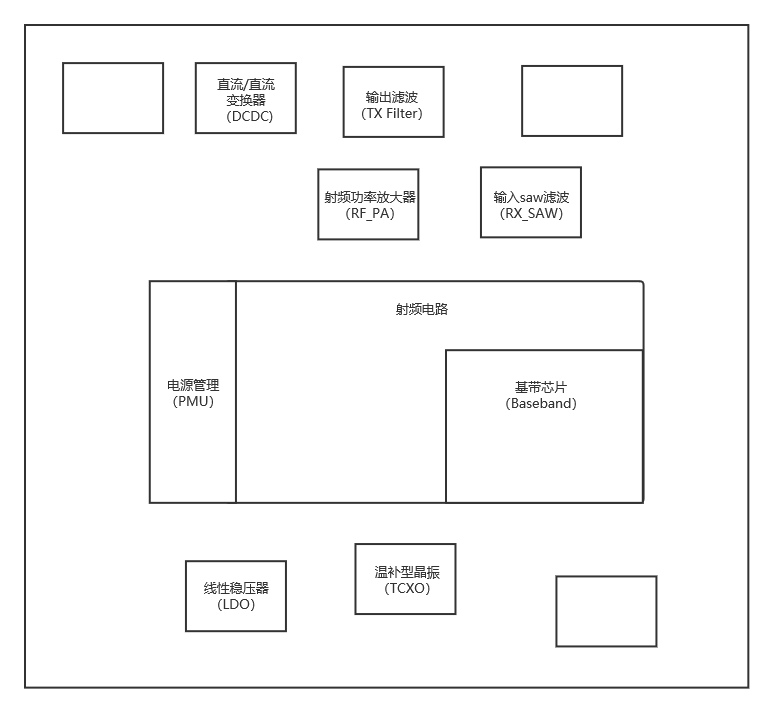
\includegraphics[width=13cm]{总体框图.png}
	\caption{总体框图}
	\label{总体框图}
\end{figure}


\section{供电}
为了将锂离子电池电压转化为模块供电电压3.1v~4.2v,选用低压降线性稳压器(LDO),具有成本低,噪音低的优点。同时由于对电池能量损耗低,保证更长的工作时间。在靠近模块的VBAT输入端,并联一个100uF的钽电容C1,以及100nF、100pF和22pF的滤波电容。同时为了提高模块承受浪涌电压的能力,在VBAT输入端增加一个TVS管D1。
输入端参考电路如图\ref{VBAT}:
\begin{figure}[H]
	\centering
	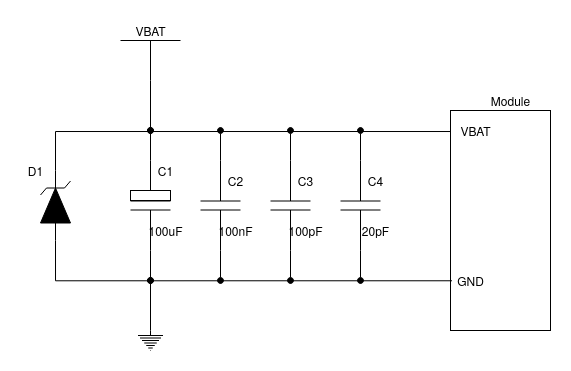
\includegraphics[width=10cm]{VBAT.png}
	\caption{VBAT}
	\label{VBAT}
\end{figure}

\section{串口}
bc35g模块提供两对串口,分别为主串口和调试串口。主串口用于AT命令的通信、数据传输,在Active、Idle和PSM模式下均可工作。模块作为DCE,连接方式为:(TODO:图片:DCT-DTE连接)
通过RS323电平转化芯片与MCU连接,为了降低串口功耗,在模块和主机之间加上1k欧姆电阻用于降低串口电流(TODO:RS232连接图)

\section{射频模块}
BC35G天线部分预留了pi型匹配电路如图\ref{ANT},以便对天线性能调节。C1和C2两个电容将大多数交流成分滤除,R1为0欧电阻,充当pi型RC滤波电路的电感。为了确保射频信号的性能以及可靠性,需要遵循pi型匹配电路的layout。既要保证电容电感布局靠近,也要防止出现stub(TODO:引用)
\begin{figure}[H]
	\centering
	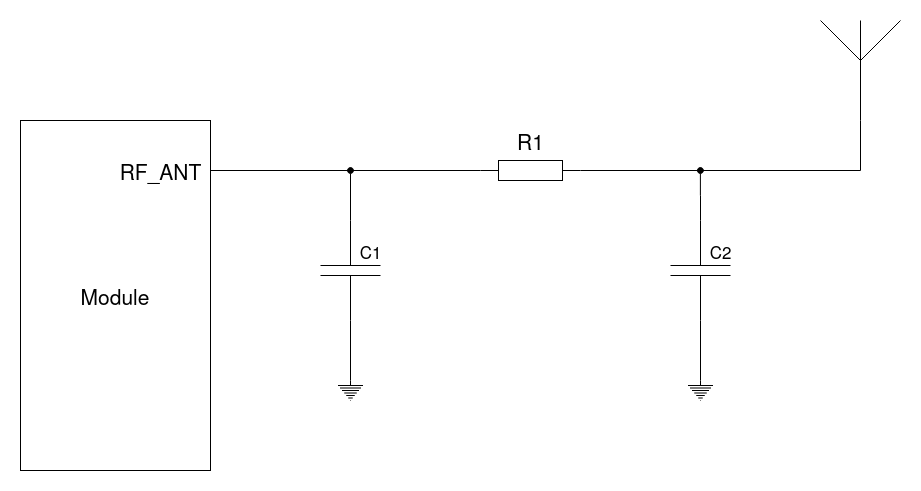
\includegraphics[width=10cm]{ANT.png}
	\caption{ANT}
	\label{ANT}
\end{figure}
\section{USIM卡座}
支持3GPP规范功能的USIM卡能接入运营商网络,USIM功能包括模块和卡座,为了确保USIM卡的性能以及避免与射频、电源模块的干扰,须遵循以下设计原则:

\begin{enumerate}
\item 卡座和模块尽量靠近,信号线不超过200mm保证信号品质
\item 信号线远离RF走线及VBAT
\item 防止USIM\_DATA和USIM\_CLK信号干扰,两线之间加入地屏蔽
\item USIM\_DATA, USIM\_VDD, USIM\_CLK, 和USIM\_RST并联33pF电容滤除RF干扰
\item 为了防止静电,在卡座和模块之间增加TVS管
\end{enumerate}

USIM卡使用内部电源3v供电,引脚定义如下

USIM卡座电路图如\ref{USIM}
\begin{figure}[H]
	\centering
	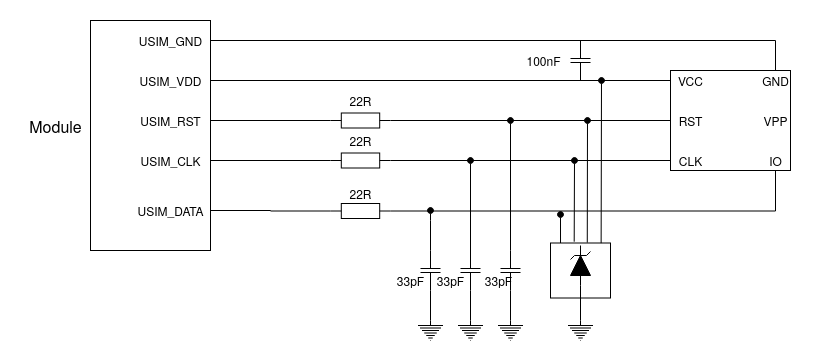
\includegraphics[width=10cm]{USIM.png}
	\caption{USIM}
	\label{USIM}
\end{figure}

\section{本章小结}

本章讨论了BC35G模块的外围电路设计,包括USIM卡座、电源、天线以及串口,主要关注于各部分之间的信号干扰避免,通过合理使用滤波电容,不同部分在电路板上的位置的相对远离,以达到良好的射频信号性能以及可靠性。同时通过TVS管等方式降低电涌对设备的损害。